\documentclass[../sparc.tex]{subfiles}
\graphicspath{{\subfix{../images/}}}
\begin{document}

%%%%%%%%%%%%%%%%%%%%%%%%%%%%%%%%%%%%%%%%%%%%%%%%%%%%%%%%%%%%%%%%%%%%%%%%%%%%%%%%
\section{Signal Types}

There are two main types of signals -- \emph{analog} and \emph{digital} signals.
To compare them to each other let's take a look on figures
\ref{fig:adc-analog-signal-example} and \ref{fig:adc-digital-signal-example}.

\begin{figure}[ht]
  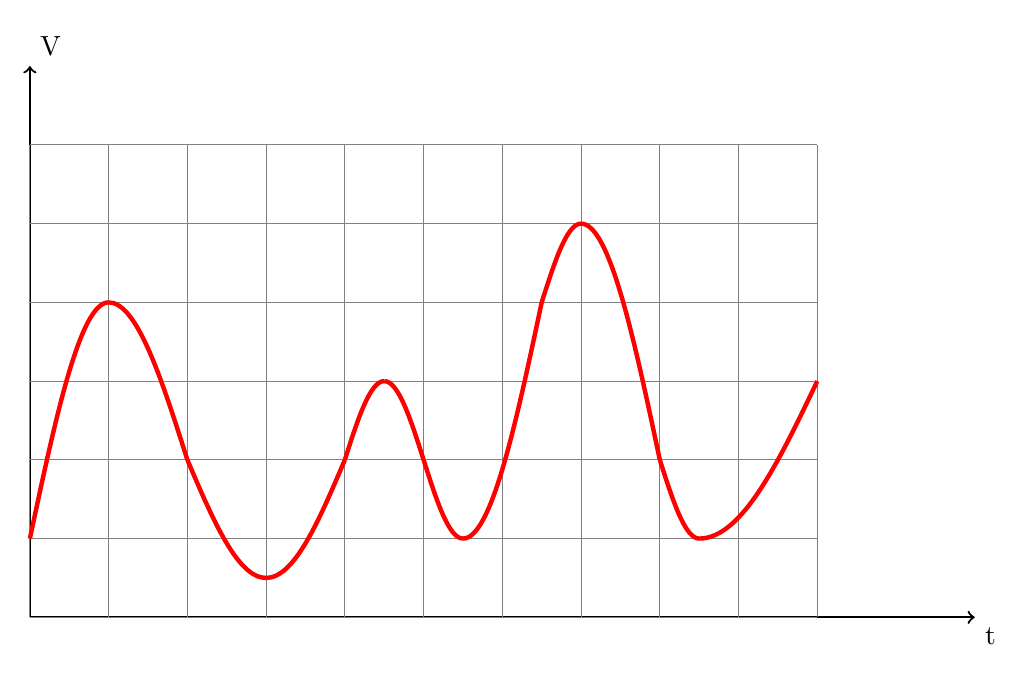
\begin{tikzpicture}
    \draw[thick, ->] (0, 0) -- (12, 0) node[anchor=north west] {t};
    \draw[thick, ->] (0, 0) -- (0,  7) node[anchor=south west] {V};
    \draw[gray] (0, 0) grid (10, 6);
    \draw[ultra thick, red] (0,1)   sin (1,4);
    \draw[ultra thick, red] (1,4)   cos (2,2);
    \draw[ultra thick, red] (2,2)   sin (3,0.5);
    \draw[ultra thick, red] (3,0.5) cos (4,2);
    \draw[ultra thick, red] (4,2)   sin (4.5,3);
    \draw[ultra thick, red] (4.5,3) cos (5,2);
    \draw[ultra thick, red] (5,2)   sin (5.5,1);
    \draw[ultra thick, red] (5.5,1) cos (6.5,4);
    \draw[ultra thick, red] (6.5,4) sin (7,5);
    \draw[ultra thick, red] (7,5)   cos (8,2);
    \draw[ultra thick, red] (8,2)   sin (8.5,1);
    \draw[ultra thick, red] (8.5,1) cos (10, 3);
  \end{tikzpicture}
  \caption{Analog signal example.}
  \label{fig:adc-analog-signal-example}
\end{figure}

\begin{figure}[ht]
  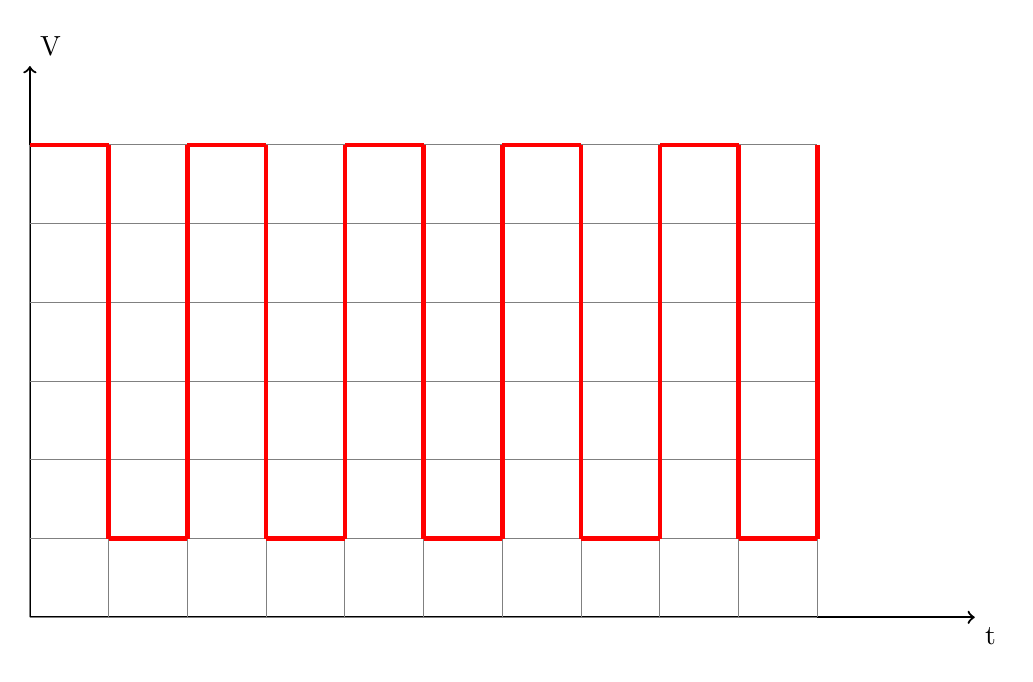
\begin{tikzpicture}
    \draw[thick, ->] (0, 0) -- (12, 0) node[anchor=north west] {t};
    \draw[thick, ->] (0, 0) -- (0,  7) node[anchor=south west] {V};
    \draw[gray] (0, 0) grid (10, 6);
    \foreach \x in {0, 2, ..., 8} {
      \draw[ultra thick, red] (\x, 6) -- (\x + 1, 6);
      \draw[ultra thick, red] (\x + 1, 6) -- (\x + 1, 1);
      \draw[ultra thick, red] (\x + 1, 1) -- (\x + 2, 1);
      \draw[ultra thick, red] (\x + 2, 1) -- (\x + 2, 6);
    }
  \end{tikzpicture}
  \caption{Digital signal example.}
  \label{fig:adc-digital-signal-example}
\end{figure}

On both graphs ``Y'' axis represents Volts and ``X'' axis represents time.

As you can see an analog signal does not have clear logical levels and changes
in time in some specified range.  On the other hand a digital signal has clear
logical levels that represent ones and zeroes.

Take a human voice as an analog signal example.  If we try to record the voice
using a digital recorder then the recorder will receive a sound wave similar to
the one that you can see on fig. \ref{fig:adc-analog-signal-example}.

For digital signals we can use a sound recording that is transferring through
the Internet as an example.  If we save a digital signal on a storage device
we'll get digital data consisting of zeroes and ones -- on conventional computers
such data is usually stored as files.

Also computers have ability to receive and \emph{digitize} analog signals.
Thanks to this ability a computer or a micro-controller can receive various
information about the world around, as many of the different environment
parameters are represented by values that don’t have fixed levels.  Examples
are: temperature, humidity, illumination, atmospheric pressure and so on.

Thus most of the micro-controllers have analog inputs for working with analog
signals and we will discuss those possibilities using Arduino platform as an
example.

But first we need to learn the tools that will give us the ability to see the
signal that is received and processed by a micro-controller.

\end{document}
